\documentclass[10pt, a4paper]{article}
\usepackage[spanish]{babel} % espanol.
%Lo pongo en english para que me compile :S.

\usepackage[utf8]{inputenc}
\usepackage{enumerate} % enumerados
\usepackage{graphicx}
\usepackage{longtable}
\usepackage{multicol}
\graphicspath{ {img/} }
\usepackage[paper=a4paper, left=1.5cm, right=1.5cm, bottom=1.5cm, top=3.5cm]{geometry}
\usepackage{indentfirst}
\usepackage{fancyhdr}
\usepackage{color}
\usepackage[colorlinks=true, linkcolor=black]{hyperref}
\usepackage{a4wide}
\usepackage{tikz}
\usepackage{epsf}
\usepackage{caratula}
\usepackage{mathtools}
\usepackage[section]{placeins}
\usepackage{etoolbox}
\preto{\section}{\clearpageafterfirst}
\preto{\subsection}{\filbreak}
\newcommand{\clearpageafterfirst}{%
  \gdef\clearpageafterfirst{\clearpage}%
}

\begin{document}


\begin{figure}[ptb]

\includegraphics[scale=0.30]{logo.jpg}\hspace{6cm}

\includegraphics[scale=0.90]{logo_dc.jpg}
\end{figure}

%Datos de la caratula
\materia{Robotica Movil}
\titulo{Trabajo pr\'actico Final}
%\subtitulo{Parser}
\hspace{6cm}
\integrante{Negri, Franco}{893/13}{franconegri2004@hotmail.com}
\integrante{Schmit, Matías}{714/11}{matias.schmit@gmail.com}
\palabrasClave{Odometria, Seguimiento Trayectorias, Cimenatica, Kalman}
  % Reconocimiento caras. PCA. Power Method. Deflation. Autovalores. Autovectores. Matriz
  % semi definida positiva.

\resumen{Segimiento de trayectorias para robot odometrico}

\parskip=5pt % 10pt es el tamaño de fuente

% Pongo en 0 la distancia extra entre ítemes.
\let\olditemize\itemize
\def\itemize{\olditemize\itemsep=0pt}

% Acomodo fancyhdr <- Creo que es el encabezado de pagina
\pagestyle{fancy}
\thispagestyle{fancy}
\addtolength{\headheight}{1pt}
%\lhead{Acosta, Negri}
%\rhead{1$^{do}$ Cuatrimestre 2016}
\cfoot{\thepage}
\renewcommand{\footrulewidth}{0.4pt}




%Pagina de titulo e indice
\thispagestyle{empty}

\maketitle



\tableofcontents
\pagebreak
\section{Introduccion}
En los ultimos años se ha visto un gran avance en el campo de la robotica y en tareas automatizables. En particular, los robots omnidireccionales se han empezado a utilizar tanto en la industria, por su capacidad de maniobrar en espacios reducidos, como en la domotica por su comodidad.

En este trabajo practico implementaremos un sistema que permita la realizacion de trayectorias de manera segura y presisa utilizando un robot omnidireccional. Para ello utilizaremos el entorno de desarrollo ROS y el entorno de simulación V-Rep.

El robot en particular sobre el cual trabajaremos contará con cuatro ruedas fijas con diseño Mecanum. De este modo, parte de nuestro trabajo será implementar un modelo cinematico acorde que nos permita tanto controlar la velocidad como estimar la velocidad lineal y angular a partir de la informacion sensada por las cuatro ruedas.

\section{Desarrollo}
\subsection{Adaptación del modelo cinemático}
%explicar que es cinemática directa e inversa
Como ya anticipamos, para este trabajo practico utilizaremos un robot omidireccional. Este cuenta con cuatro ruedas  \textit{Mecanum} dispuestas a los costados del robot, las cuáles cuentan con rodillos especiales que permiten transmitir parte de la fuerza en dirección de un ángulo definido.  %agregar mas detalles sobre las ruedas que estan en el abstract del paper


El primer desafío que se nos presenta ante este nuevo sistema es poder plantear el modelo cinemático del mismo, recordemos que en el contexto de este trabajo la cinemática es el estudio de cómo se comporta el robot en movimiento y el aporte de cada rueda en este sistema basándose en los inputs de control, el movimiento esperado y sin considerar las fuerzas que se aplican.

Considerando la relación entre inputs y movimiento esperado queda definida la cinemática directa como la obtención de la velocidad lineal y angular (expresada en m/s y radianes respectivamente) del robot a partir de la velocidad de cada actuador.

Por su parte la cinemática inversa determina la velocidad de los actuadores en base a la velocidades deseadas.

Para lograr esto, adaptaremos el modelo cinemático visto durante la materia utilizando el paper provisto por la cátedra, las formulas de cinemática directa pasarán a ser.

$$v_x(t)=(w_1+w_2+w_3+w_4).r/4$$
$$v_y(t)=(-w_1+w_2+w_3-w_4).r/4$$
$$w_z(t)=(-w_1+w_2-w_3+w_4).r/(4(l_x+l_y))$$


Y las de cinemática inversa:

$$ w_1 = 1/r (v_x - v_y - (l_x + l_y)w_z$$
$$ w_2 = 1/r (v_x + v_y + (l_x + l_y)w_z$$
$$ w_3 = 1/r (v_x + v_y - (l_x + l_y)w_z$$
$$ w_4 = 1/r (v_x - v_y + (l_x + l_y)w_z$$

%se podria hacer una lista.
Donde el Vector V = ($v_x$, $v_y$ y $w_z$) refiere a las velocidades lineares y angular del robot, $r$ el radio de las ruedas (todas las ruedas tienen exactamente el mismo radio), $l_x$ la mitad de la distancia entre las dos ruedas delanteras y $l_y$ la mitad de la distancia entre una rueda delantera y una rueda trasera.En particular para nuestro robot sabemos que $r =50 $ mm, $l_x = l_y = 175 $ mm. Por último $w_1,w_2,w_3,w_4$ representan las velocidades angulares ejercidas por los actuadores de las ruedas.

Finalmente con las velocidades obtenidas en $v_x$, $v_y$ y $w_z$ podremos estimar la pose del robot en cada instante calculando el desplazamiento en el tiempo que las velocidades nos proveen.

Si bien esto nos permitirá estimar la pose del robot, a causa de los errores sistemáticos del modelo utilizado, el error entre la pose real y la pose estimada divergirá con el tiempo. 


En el siguiente apartado procederemos a analizar cuan bueno resulta nuestro modelo cinemático y los cálculos odométricos.

\subsubsection{Experimentación}

Como ya adelantamos, en este apartado buscaremos ver que tan exacto resulta nuestro modelo cinemático y la odometría calculada de manera experimental. Para ello, enviaremos mensajes a robot\/cmd\_vel a través de rostopic con distintas consignas de velocidad y veremos por RViz cual es la posición calculada por odometría (base\_link) y cual es la posición real del robot (base\_link\_gt). 


Como primer experimento enviamos el comando de velocidad $(v_x = 2, v_y=0, w_z=0)$ durante $8$ segundos:

\begin{center}
\begin{figure}[!htb]
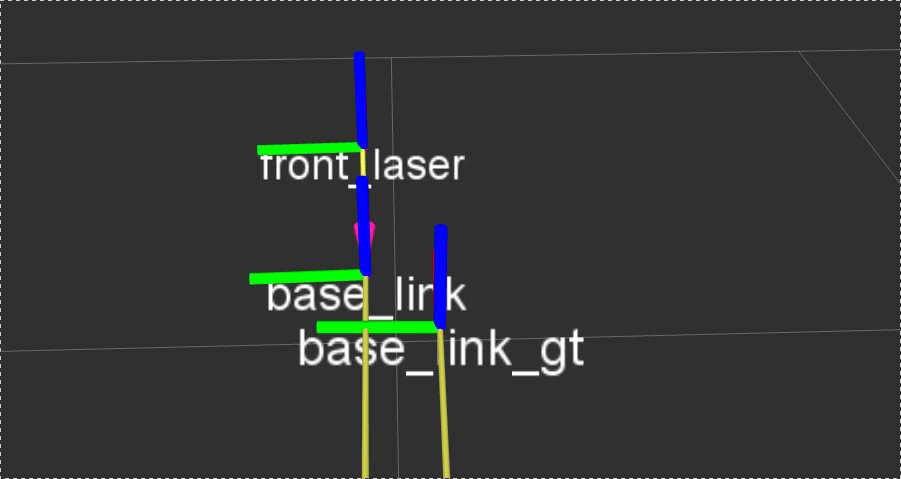
\includegraphics[width=\linewidth]{pruebasOdom/8segAdelante2.png}
\end{figure}
\FloatBarrier
\end{center}

Podemos observar que incluso a altas velocidades el modelo es capaz de predecir con bastante exactitud su posición.

Para el siguiente experimento, enviamos la consigna de velocidad $(v_x = 0, v_y=2, w_z=0)$ durante $8$ segundos.

\begin{center}
\begin{figure}[!htb]
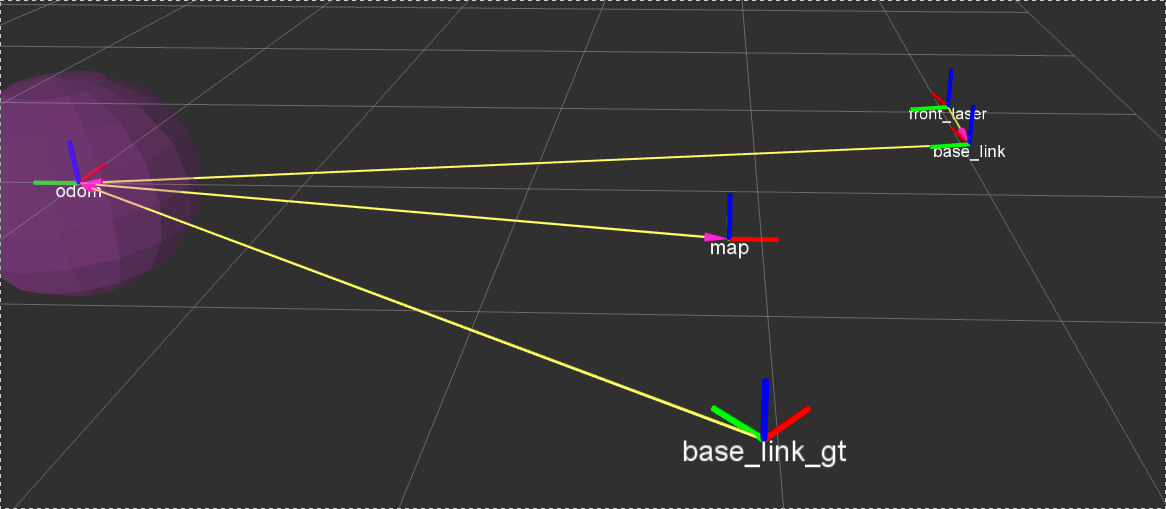
\includegraphics[width=\linewidth]{pruebasOdom/8segIzquierda2.png}
\end{figure}
\FloatBarrier
\end{center}
En este caso, podemos ver que la estimación odometrica diverge ampliamente con la provista por el simulador, incluso en vez de realizar una trayectoria recta hacia uno de los costados realiza una elipse. Esto puede deberse principalmente a que los rodillos especiales que le permiten trasladarse en el eje $y$ resbalan o que los actuadores no logran cumplir la consigna deseada. Para el siguiente experimento volvemos a realizar el mismo experimento pero reduciendo la velocidad deseada.

Enviando la consigna $(v_x = 0, v_y=0.5,w_z=0)$ durante 8 segundos: 

\begin{center}
\begin{figure}[!htb]
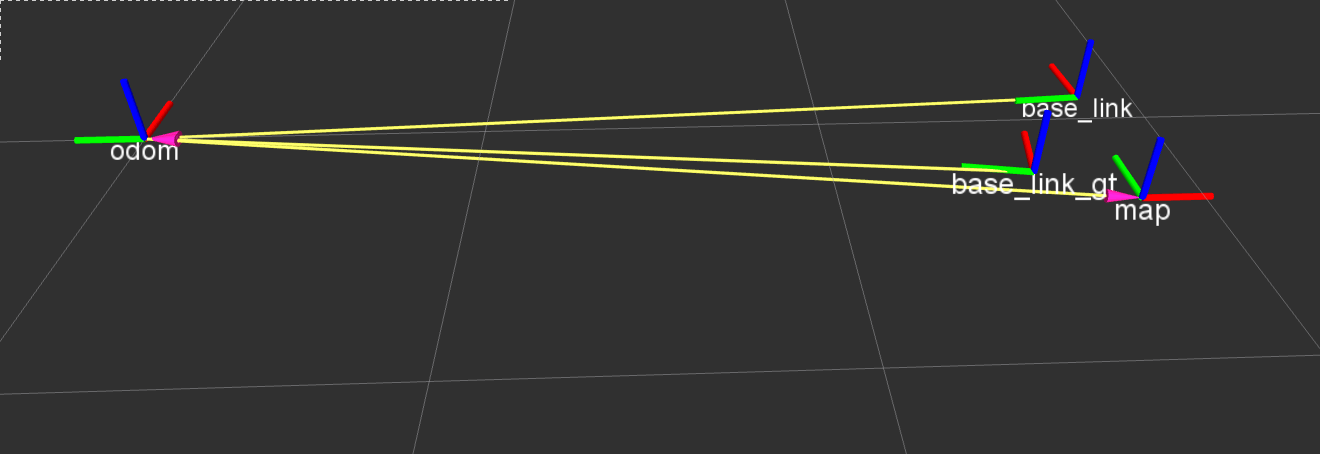
\includegraphics[width=\linewidth]{pruebasOdom/8segIzquierda05.png}
\end{figure}
\FloatBarrier
\end{center}
Podemos ver que para velocidades menores la calidad de las predicciones odométricas son mucho mejores, aún así puede verse que en este eje el error crece mucho mas rápido que en el eje $x$.

\pagebreak

Para finalizar enviamos como consigna $(v_x = 0, v_y=0,w_z=2)$, luego de realizar 3 vueltas sobre su eje, detenemos al robot y visualizamos en RViz:

\begin{center}
\begin{figure}[!htb]
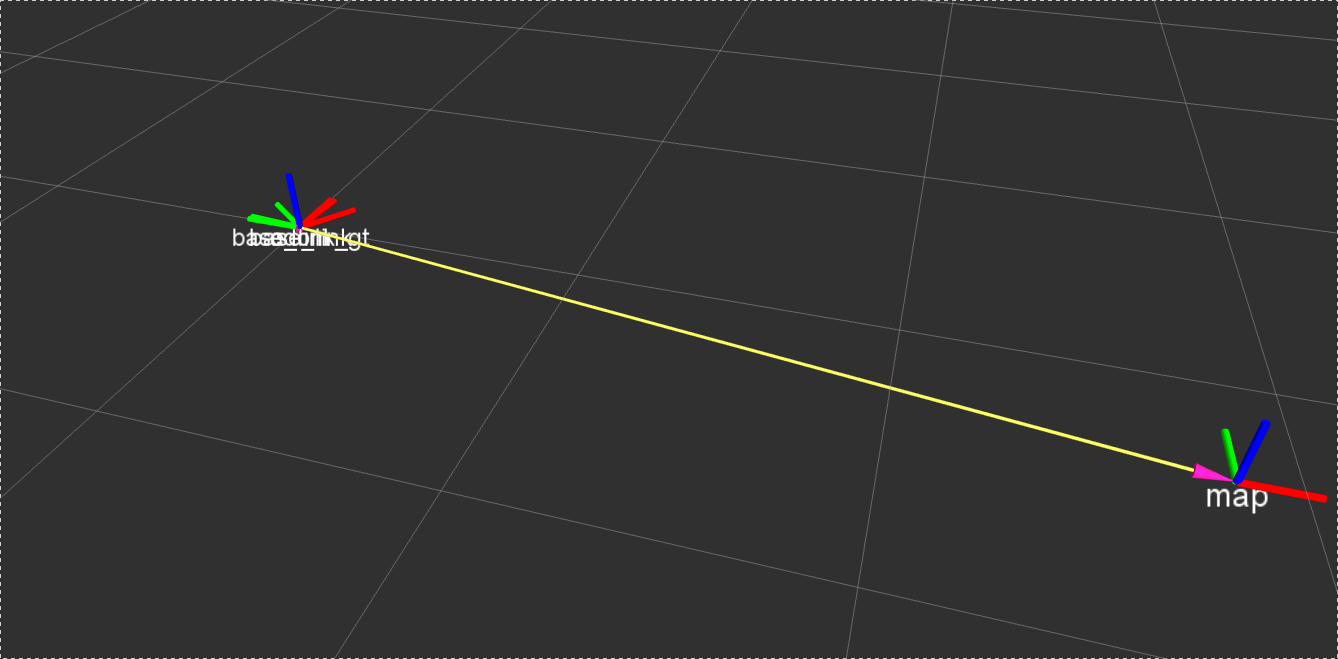
\includegraphics[width=\linewidth]{pruebasOdom/3Vueltas2Vel.png}
\end{figure}
\FloatBarrier
\end{center}
Puede verse que el error en este caso tampoco crece de manera desproporcionada incluso exigiéndole altas velocidades.


% Plantear experimentos que permitan validar y evaluar la efectividad del modelo. Entre los experimentos a realizar se deben incluir graficos de consignas de velocidades lineales y angular del robot junto a las correspondientes velocidades reales ejercidas por el robot, para su comparaci ́on. Asimismo, se debe incluir un grafico que permita comparar la pose del robot estimada seg un odometria con la real informada por el simulador.

\subsection{Adaptación del control a lazo cerrado}

%Este parrafo puede ir antes cuando mencionamos errores sistematicos o aca
Así como encontramos errores sistemáticos intrínsecos al diseño del robot, vale la pena destacar que por fuera del entorno simulado en el que estamos probando el modelo, también nos encontraríamos con errores no sistemáticos del entorno que harían aun menos confiable a nuestra estimación odometrica. Sumando a consideración la experimentación y esto último es necesario seguir agregando funcionalidades a nuestro modelo que permita mejorar la precisión en el desplazamiento. 

Al igual que para el robot con modelo diferencial queremos que este se pueda trasladar de una pose actual $(x_i,y_i,w_i)$ en un tiempo $t_i$ a una pose objetivo $(x_f,y_f,w_f)$ en un tiempo diferente $t_f$. Para eso utilizaremos un control a lazo cerrado basado en el controlador Proporcional Integrativo Derivativo (PID) que nos permitirá observar si el robot se encuentra en la pose deseada en cada instante, retroalimentando el error a los controladores de velocidad.

En este caso, al tener un modelo cinemático holonómico las cuentas se simplifican con respecto al modelo diferencial, el control independiente sobre cada velocidad permite plantear cada  dimensión por separado:

$$\Delta_x = x_f - x_i / (t_f - t_i)$$
$$\Delta_y = y_f - y_i / (t_f - t_i)$$
$$\Delta_w = w_f - w_i / (t_f - t_i)$$

Donde $\Delta_x$, $\Delta_y$ y $\Delta_w$ es la diferencia entre la pose actual y la objetivo. Minimizar esto significará haber alcanzado la pose objetivo, por lo que definimos las velocidades del robot como:

$$V_x = K \Delta_x $$
$$V_y = K \Delta_y $$
$$\theta = K \Delta_w $$

Donde $K$ es una constante proporcional.
%aca podemos mencionar PID y como esta implementado en este modelo. 
%el termino proporcional se encarga de ajustar el error inmediato buscando llevar la diferencia en estado estacionando a cero.
%el termino integral acumula los errores obtenidos hasta ese punto 
%el termino derivativo utiliza el error para estimar diferencias a futuro

%porque no se usaban el termino integral y derivativo?   

Nos queda solucionar un caso borde que se da si la pose actual y la objetivo se encuentran a una distancia infinita (o cercana a infinita), en este caso será necesaria una velocidad infinita para alcanzarla. Dado que esto no es físicamente posible, definimos una cota máxima de velocidad.

%Cual era la cota de velocidad ?

\subsubsection{Experimentación}

A continuación se pone a prueba el control a lazo cerrado:

Para ello pondremos al robot a realizar el seguimiento de una trayectoria cuadrada de 2 metros de lado y veremos cual es el comportamiento del robot tomando $K=0.4,1$ y $4$ y visualizandolo en r-viz.

$K = 0.4$

\begin{figure}[!htb]
\minipage{0.32\textwidth}
  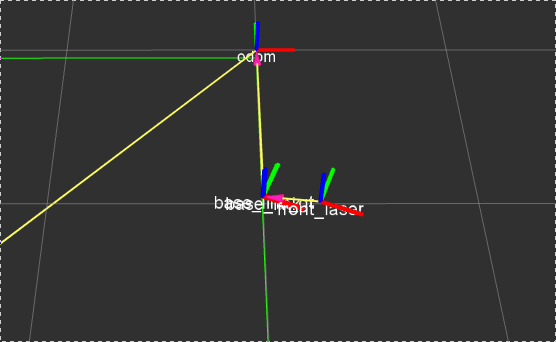
\includegraphics[width=\linewidth]{imagenesExpLazoCerrado/k0.4/1.png}
\endminipage\hfill
\minipage{0.32\textwidth}
  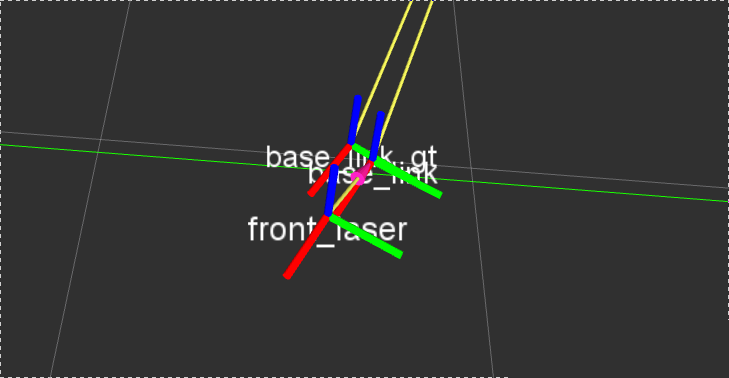
\includegraphics[width=\linewidth]{imagenesExpLazoCerrado/k0.4/3.png}
\endminipage\hfill
\minipage{0.32\textwidth}%
  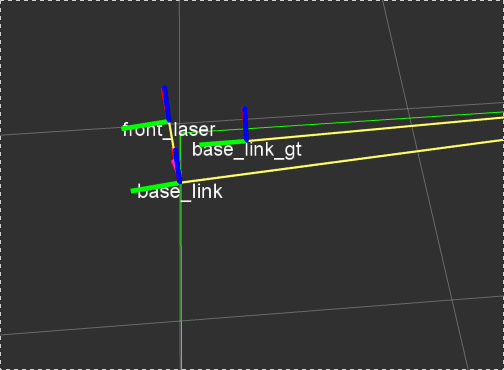
\includegraphics[width=\linewidth]{imagenesExpLazoCerrado/k0.4/5.png}
\endminipage
\end{figure}
\FloatBarrier

Como otra metodología de visualización, logeamos las poses provenientes del ground truth provistas por roscore y los graficamos de la siguiente manera:

% insertar grafico 
\begin{figure}[!htb]
\begin{center}
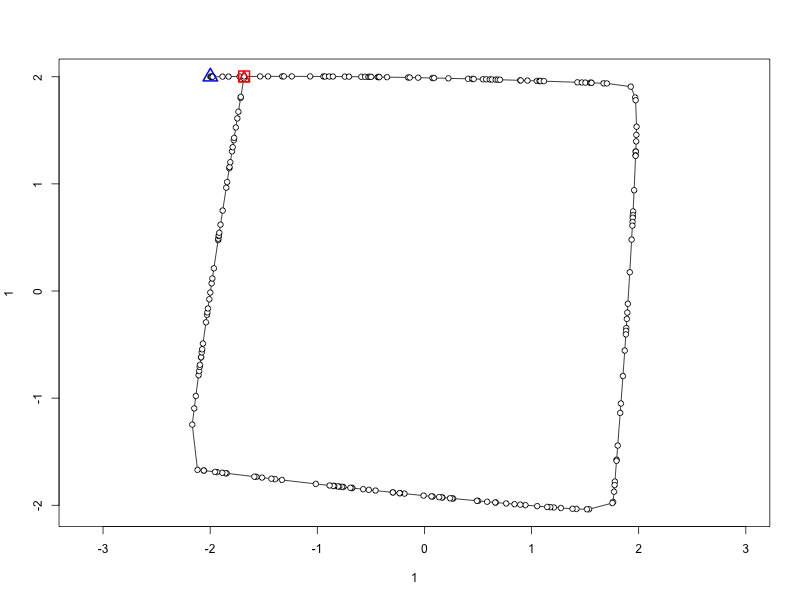
\includegraphics[width=\linewidth/2]{imagenesTrayectorias/lazocerrado/lazocerrado04.png}
\end{center}
\end{figure}
\FloatBarrier

$K = 1$

\begin{figure}[!htb]
\minipage{0.32\textwidth}
  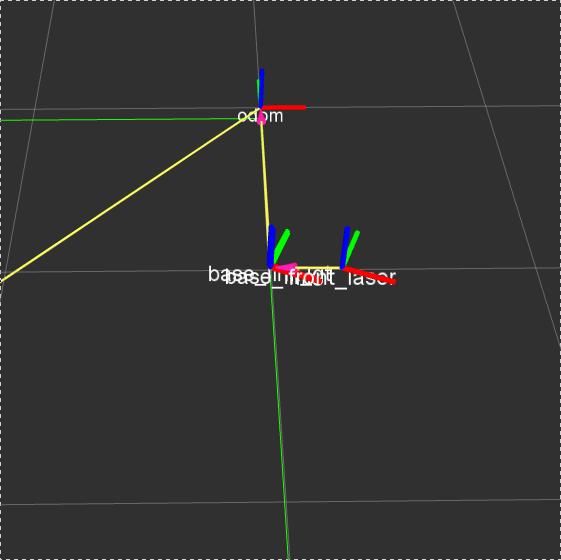
\includegraphics[width=\linewidth]{imagenesExpLazoCerrado/k1/1.png}
\endminipage\hfill
\minipage{0.32\textwidth}
  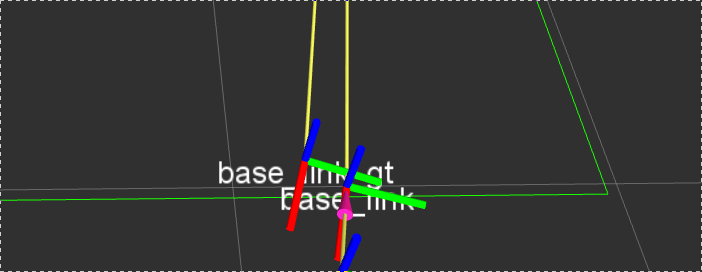
\includegraphics[width=\linewidth]{imagenesExpLazoCerrado/k1/3.png}
\endminipage\hfill
\minipage{0.32\textwidth}%
  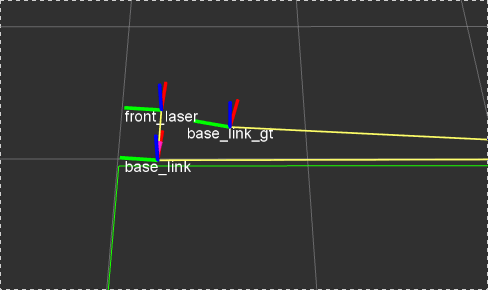
\includegraphics[width=\linewidth]{imagenesExpLazoCerrado/k1/5.png}
\endminipage
\end{figure}
\FloatBarrier

% insertar grafico 
Trayectoria Efectiva:

\begin{figure}[!htb]
\begin{center}
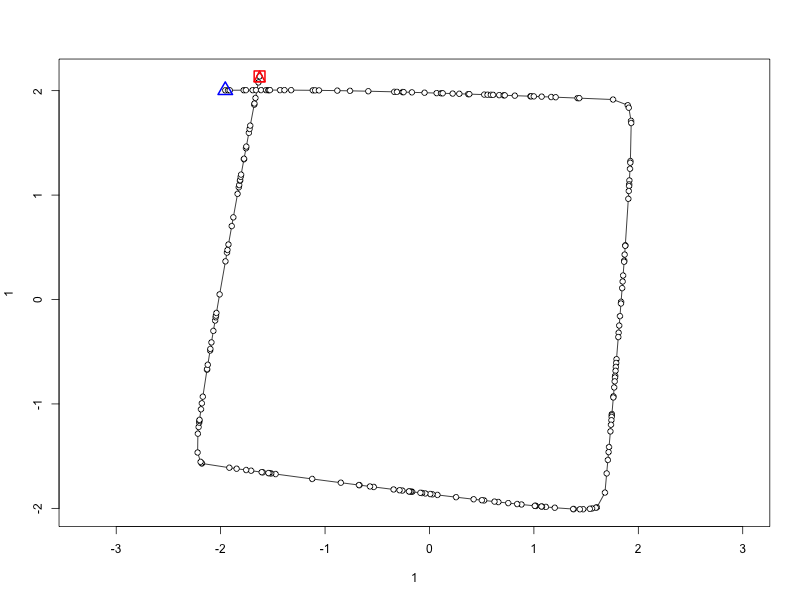
\includegraphics[width=\linewidth/2]{imagenesTrayectorias/lazocerrado/lazocerrado1.png}
\end{center}
\end{figure}
\FloatBarrier


\pagebreak
$K = 4$


\begin{figure}[!htb]
\minipage{0.32\textwidth}
  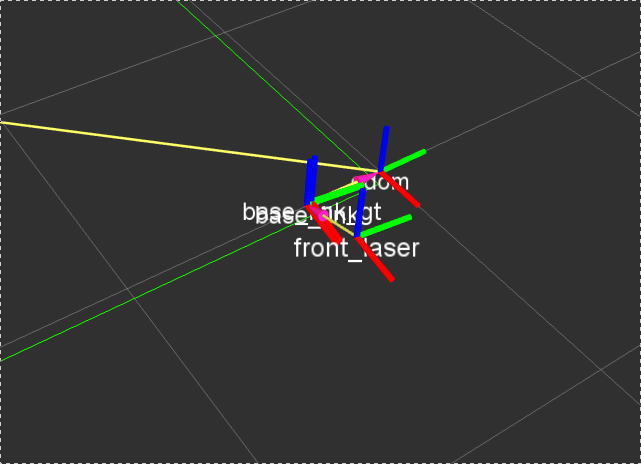
\includegraphics[width=\linewidth]{imagenesExpLazoCerrado/k4/1.png}
\endminipage\hfill
\minipage{0.32\textwidth}
  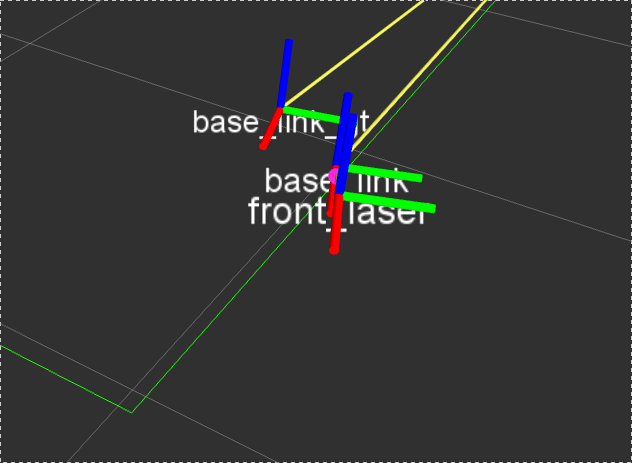
\includegraphics[width=\linewidth]{imagenesExpLazoCerrado/k4/2.png}
\endminipage\hfill
\minipage{0.32\textwidth}%
  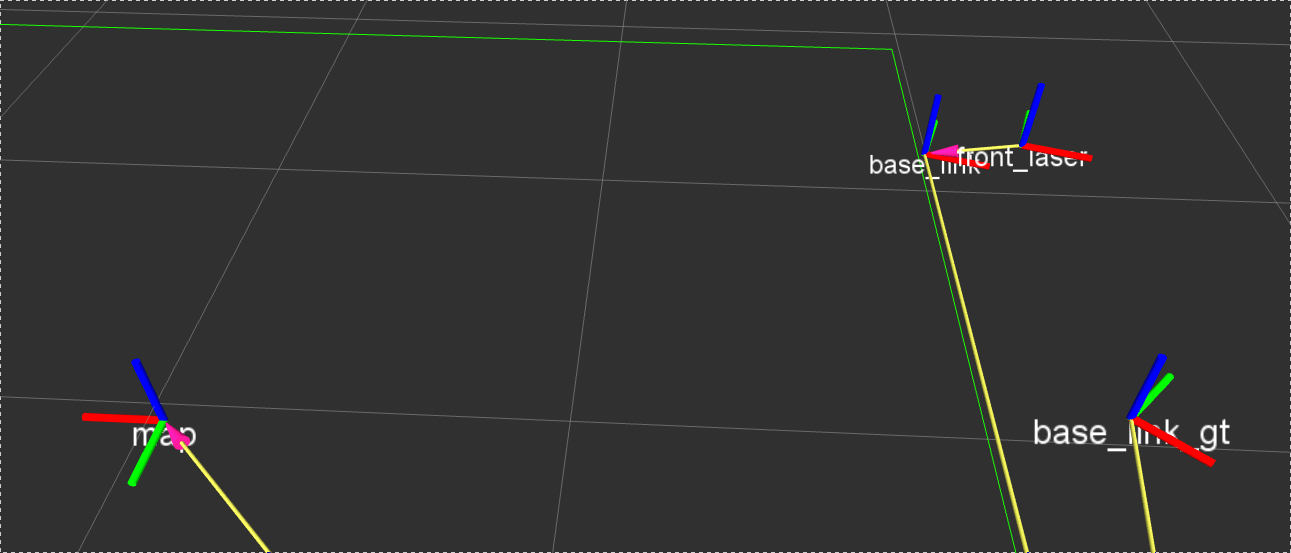
\includegraphics[width=\linewidth]{imagenesExpLazoCerrado/k4/4.png}
\endminipage
\end{figure}
\FloatBarrier

Trayectoria Efectiva:

% insertar grafico 
\begin{figure}[!htb]
\begin{center}
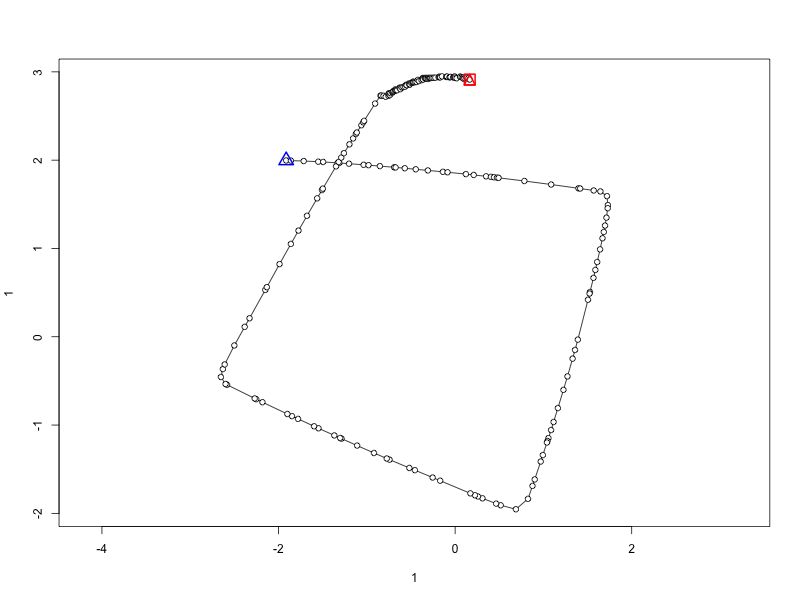
\includegraphics[width=\linewidth/2]{imagenesTrayectorias/lazocerrado/lazocerrado4.png}
\end{center}
\end{figure}
\FloatBarrier

En estas imágenes podemos notar que si bien el robot sigue la trayectoria respecto a su posición estimada de manera precisa, la estimación de la posición pierde precisión a medida que aumentamos el valor de K y observamos que para cualquier valor mayor a 1 diverge de la trayectoria esperada muy rápido. Consideramos que esto se debe a que a grandes velocidades, el modelo cinemático acumula error más rápidamente y por eso cada posición va empeorando respecto a la esperada.

\subsection{Modelado de EKF}

Como solución al problema presentado en el apartado anterior, intentaremos mejorar la corrección de la pose del robot agregando un fase de predicción del estado en el cual se encuentra.

Para eso utilizaremos un filtro bayesiano implementando el Filtro de Kalman Extendido similar al visto en la materia para el modelo diferencial.

Lo que está ocurriendo, en resumen, es que el robot usará información del censado de un serie de postes ubicados en el entorno para ir actualizando el nivel de certidumbre respecto a la ubicación en la que se encuentra. Partiendo de un \textit{prior} inicial el modelo queda definido por un fase de predicción (\textit{time update}) donde se obtienen estimaciones del estado y la covarianza del error y otra fase de corrección (\textit{measurement update}) donde se actualizan los valores de la fase anterior con las mediciones obtenidas, el \textit{posterior} obtenido pasa a ser nuestro nuevo \textit{prior} y el algoritmo continua iterando de forma análoga.


Partiendo de las funciones que definen ubicación y censado tenemos:

$x_k = f(x_{k-1}, u_{k-1},w_{k-1}) + w_k$  (Proyección de la pose actual en función de una $f$ de transición sobre la iteración anterior y la consideración del ruido w)

$z_k = h(x_{k-1},v_{k-1}) + v_k$   (Estado del censado a partir de una función $h$ sobre la iteración anterior considerando ruido del sensor v )

El siguiente diagrama expresa el funcionamiento del EKF:

%diagrama EKF en apunte kalman_notes01.pdf  -> KalmanEsquema.png
% insertar grafico 

\begin{center}
\begin{figure}[!htb]
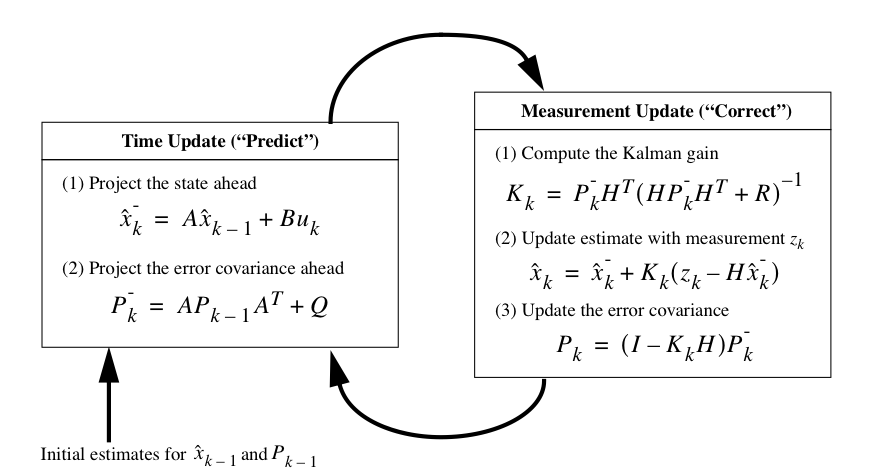
\includegraphics[width=\linewidth]{KalmanEsquema.png}
\end{figure}
\FloatBarrier
\end{center}

Las variables presentes en el modelo son: 

\begin{itemize}
\item Vector x (estado en el que se encuentra el sistema)
\item Matriz P (Error de la covarianza)
\item Matriz Q (covarianza del ruido en la transición (process))
\item Matriz R (covarianza del ruido en el censado (measurement))
\item Matriz W (Jacobiano de las derivadas parciales de f respecto a w (error en el calculo del estado))
\item Matriz A (Jacobiano de las derivadas parciales de f respecto a x (estado))
\item Matriz V (Jacobiano de las derivadas parciales de h respecto a v (error de medición))
\item Matriz H (Jacobiano de las derivadas parciales de h respecto a x (estado))
\end{itemize}
Por ultimo K se denomina \textit{ganancia de Kalman} y representa el nivel de ponderación que se le da a la información del censado por sobre la predicción estimada.

En este caso de lo que teníamos en el robot diferencial en el modelo de predicción ahora contamos con más grados de libertad posibles en la translación. Ahora es posible que el robot se mueva tanto en $x$ como en $y$ y $\theta$.

Por este motivo, el vector $\overrightarrow{u}$ que representa las entradas de control cambia de la siguiente manera:

$$\overrightarrow{u} = \begin{bmatrix}
         Vx \\
         Vy \\
         w 
        \end{bmatrix}$$


El modelo de estado $\overrightarrow{x}$ se mantiene, ya que el robot permanece igual a la del modelo anterior:

$$\overrightarrow{x} = \begin{bmatrix}
         x \\
         y \\
         \theta 
        \end{bmatrix}$$

Dada la modificación en $\overrightarrow{x}$, ahora el modelo de movimiento $f(\overrightarrow{x},\overrightarrow{u}, \overrightarrow{w})$ ahora pasará a ser:

$$f(\overrightarrow{x},\overrightarrow{u}, \overrightarrow{w})= \begin{bmatrix}
         x + Vx \Delta t cos(\theta) + Vy \Delta t sen(\theta) + w_1 \\
         y + Vx \Delta t sen(\theta) + Vy \Delta t cos(\theta) + w_2 \\
         norm_{[-\pi,\pi]} (\theta + w \Delta t) + w_3
         \end{bmatrix}$$

Calculando los jacobianos de la función $f$ respecto a $\overrightarrow{x}$ y a $\overrightarrow{w}$ respectivamente, tenemos:

$$A= \begin{bmatrix}
         1 & 0 & -sen(\theta)\Delta x + cos(\theta) \Delta t V y\\
         1 & 0 & -cos(\theta)\Delta x - sen(\theta) \Delta t V y \\
         0 & 0 & 1
         \end{bmatrix}$$

$$W$$

El modelo de censado $h(\overrightarrow{x},\overrightarrow{v})$ y las mediciones $z$ al no depender del tipo de movimiento que el robot omnidireccional ejerce no cambian, así que permanecen con los valores definidos por defecto iguales a los del modelo diferencial. De la misma forma la matriz Jacobiana H tampoco presenta cambios.

%TODO: Hablar sobre la experimentación que pide sobre modificar la covarianza inicial. Sobre esto lo unico que hay para mencionar es que se experimento con distintos niveles de covarianza inicial tanto para sensado como para movimiento pero en ambos casos el valor se estabiliza en pocas iteraciones.

%Algo así:
%"Considerando estas variables de control se experimento variando las matrices de incertidumbre inical tanto para el modelo de sensado como para el de movimiento, no hay desarrollo sobre esto en la seccion de Experimentacion (se presenta a continuacion) ya que no se encontraron resultados interesantes, el nivel de convergencia es bastante alto y con pocas iteraciones Kalman converge a partir de los datos del entorno"

\subsubsection{Experimentación}

En esta sección buscamos experimentar que tan bueno resulta el modelo EKF con las modificaciones descriptas previamente.

Partiendo de un punto en el que el robot se encuentra frente a tres postes, podemos observar que logra estimar su posición con una matriz de covarianza (en azul) casi nula.

\begin{figure}[!htb]
\begin{center}
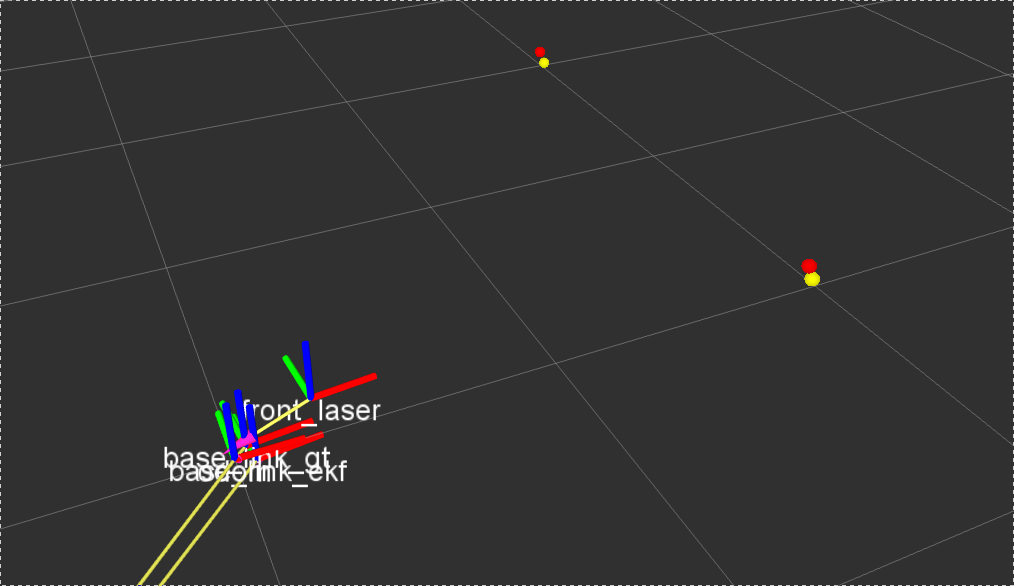
\includegraphics[scale=0.3]{punto4/ekfViendoTodosLosPostes.png}
\end{center}
\end{figure}
\FloatBarrier

\FloatBarrier

Reduciendo la distancia entre los postes y el robot, si este solo percibe dos al mismo tiempo su covarianza continúa siendo casi imperceptible en la imagen.

\begin{figure}[!htb]
\begin{center}
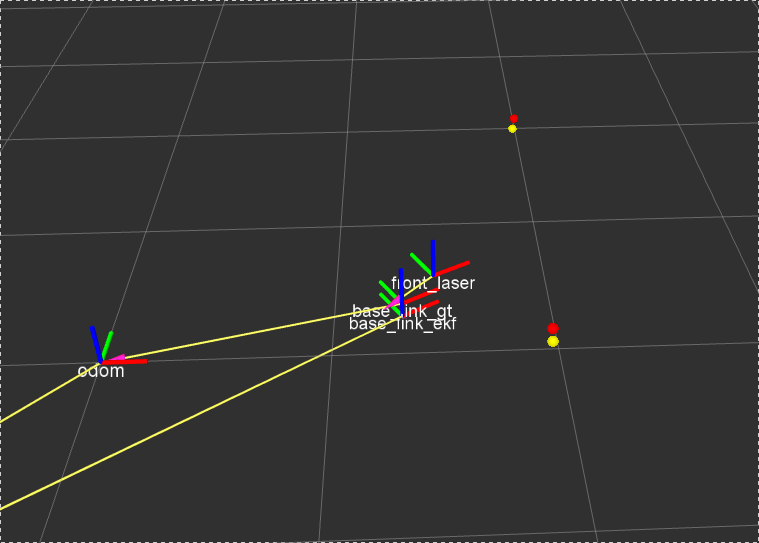
\includegraphics[scale=0.3]{punto4/ekfViendoDosPostes.png}
\end{center}
\end{figure}
\FloatBarrier


Ahora posicionando el robot para que solo cense un poste, el grado de certeza decae considerablemente. Dado que ahora solo tenemos la referencia al eje $x$ la covarianza en el eje $y$ empieza a aumentar haciendo perceptible el elipsoide violeta ensanchándose sobre ese eje.

\begin{figure}[!htb]
\begin{center}
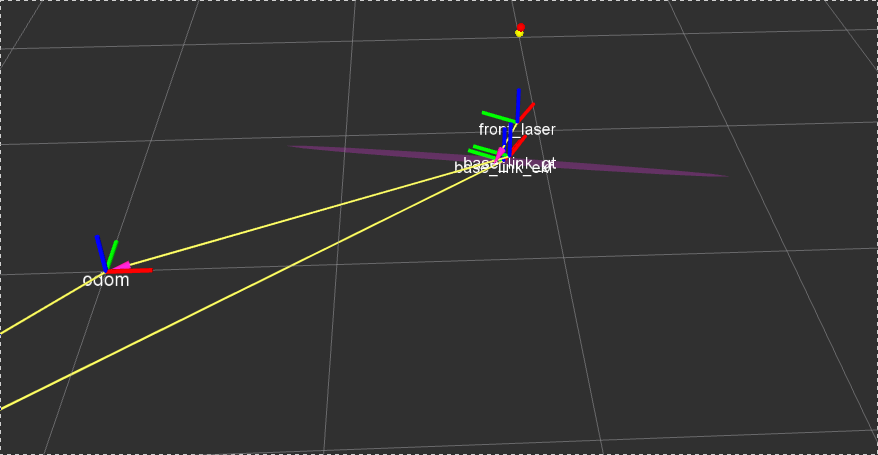
\includegraphics[scale=0.3]{punto4/ekfViendoUnPoste.png}
\end{center}
\end{figure}
\FloatBarrier

Si ahora volvemos a censar dos postes podemos observar como el robot tiene la posibilidad de recuperarse y volver a conseguir una predicción precisa de su posición, la covarianza en el eje $y$ se reduce a valores parecidos a los que teníamos antes.

\begin{figure}[!htb]
\begin{center}
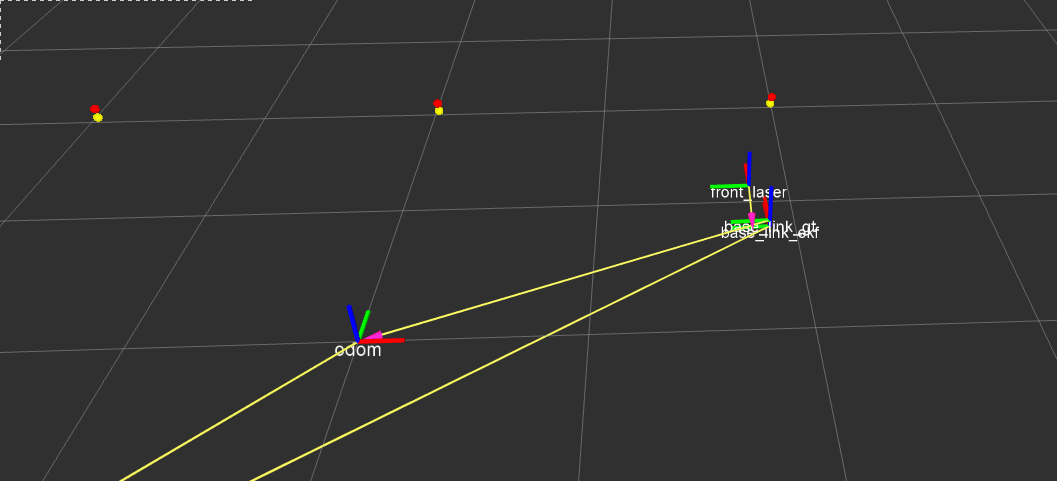
\includegraphics[scale=0.3]{punto4/ekfViendoTresPostesOtraVez.png}
\end{center}
\end{figure}
\FloatBarrier

Finalmente, si el robot no es capaz de censar ningún poste, la covarianza tanto en $x$ como en $y$ aumenta.

\begin{figure}[!htb]
\begin{center}
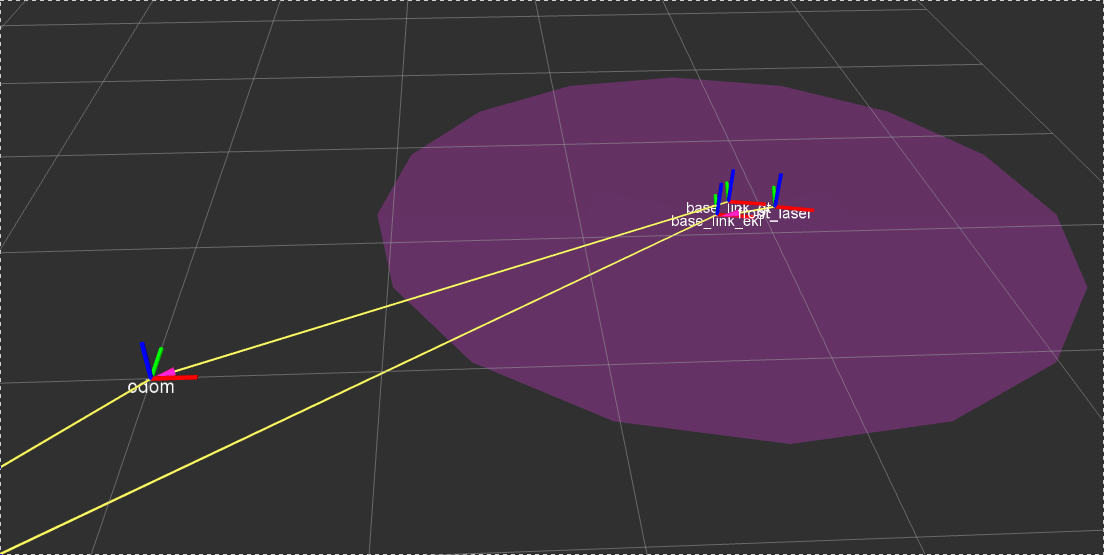
\includegraphics[scale=0.3]{punto4/ekfSinVerNingunPoste.png}
\end{center}
\end{figure}
\FloatBarrier

\section{Seguimiento de trayectorias a lazo cerrado utilizando localización basada en EKF}

En este apartado volvemos a poner a prueba el robot en el circuito previamente realizado con la trayectoria a lazo cerrado.

Nuevamente utilizamos RViz para visualizar el error y probamos con $K= 0.4,1$ y $4$:

Para $K=0.4$:

\begin{figure}[!htb]
\minipage{0.32\textwidth}
  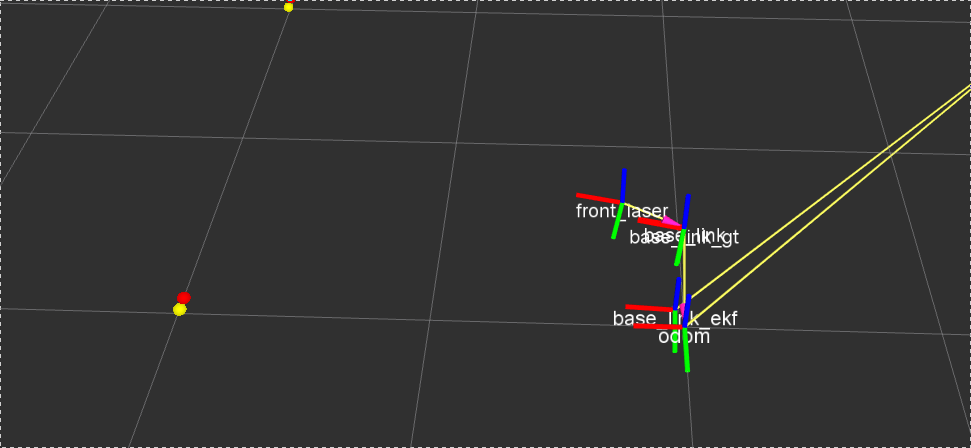
\includegraphics[width=\linewidth]{imagenesEKF/k0.4/1.png}
\endminipage\hfill
\minipage{0.32\textwidth}
  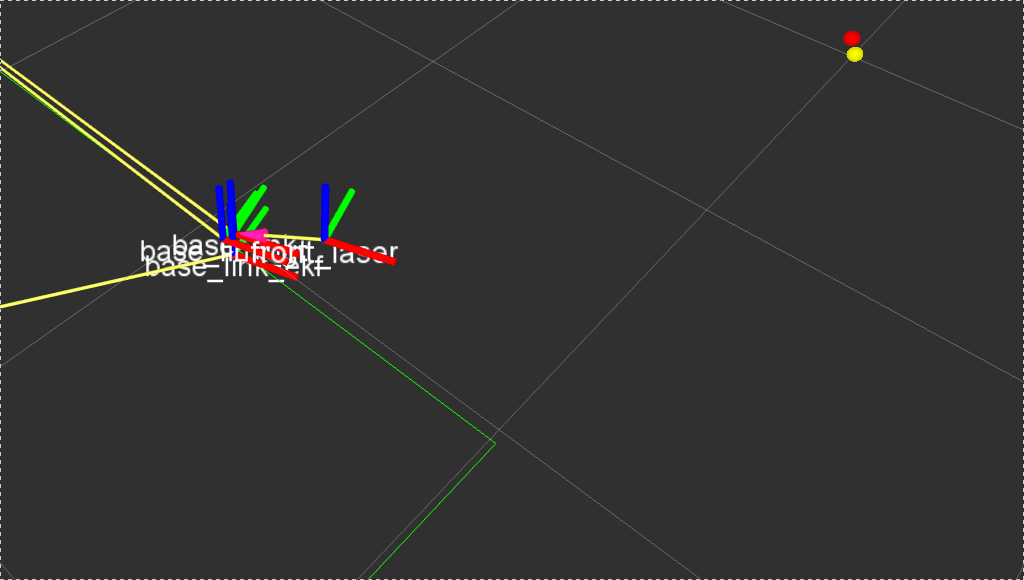
\includegraphics[width=\linewidth]{imagenesEKF/k0.4/2.png}
\endminipage\hfill
\minipage{0.32\textwidth}%
  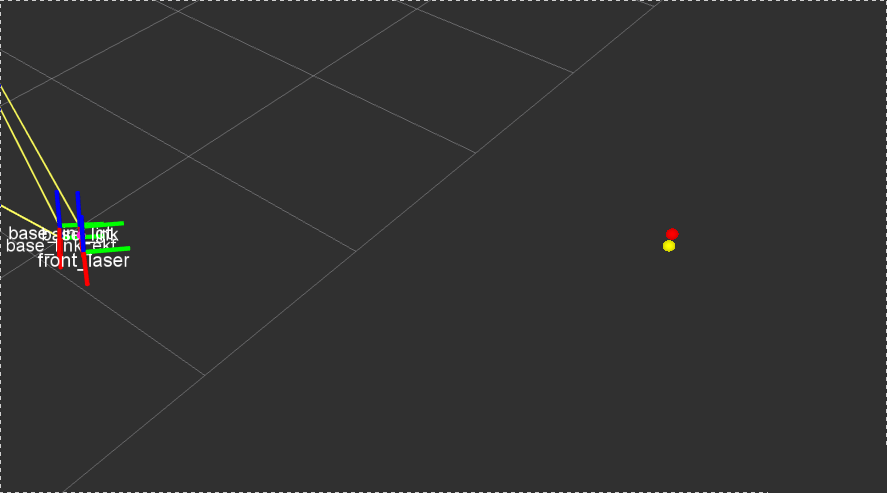
\includegraphics[width=\linewidth]{imagenesEKF/k0.4/3.png}
\endminipage
\end{figure}
\FloatBarrier

Trayectoria Efectiva:

\begin{figure}[!htb]
\begin{center}
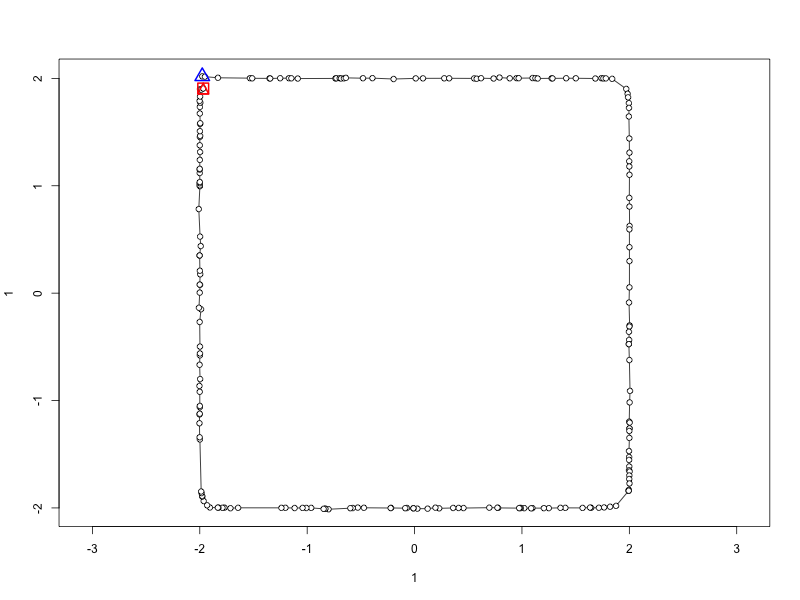
\includegraphics[width=\linewidth/2]{imagenesTrayectorias/ekf/ekf04.png}
\end{center}
\end{figure}
\FloatBarrier


En este caso podemos ver que el base\_link\_ekf permanece casi pegado al ground\_truth durante todo el recorrido. Además contamos con el base\_link (estimación odometrica sin utilizar EKF) para analizar de manera comparativa con los otros dos valores. En este caso en particular, el base\_link no se aparta demasiado de los otros dos valores.

Repetimos el experimento para $K=1$:

\begin{figure}[!htb]
\minipage{0.32\textwidth}
  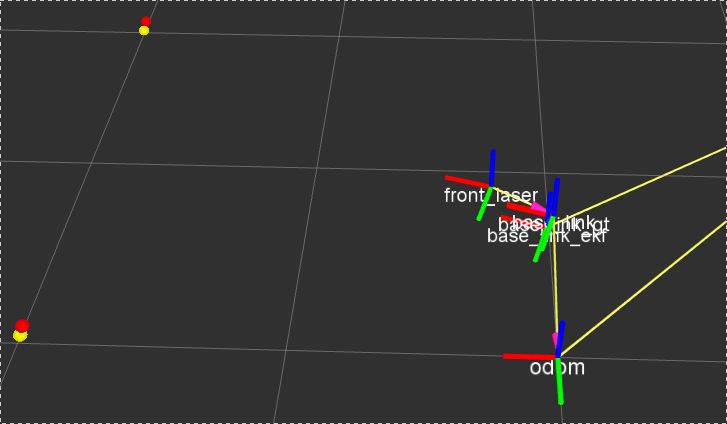
\includegraphics[width=\linewidth]{imagenesEKF/K1/1.png}
\endminipage\hfill
\minipage{0.32\textwidth}
  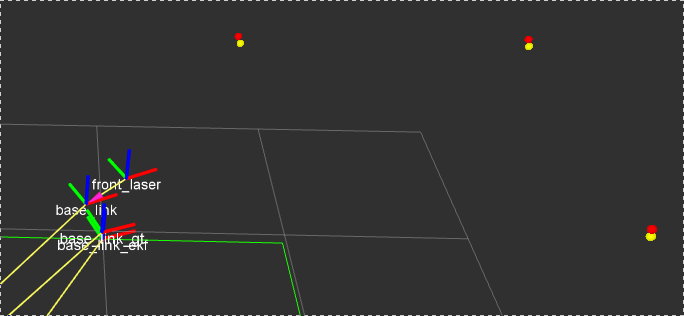
\includegraphics[width=\linewidth]{imagenesEKF/K1/3.png}
\endminipage\hfill
\minipage{0.32\textwidth}%
  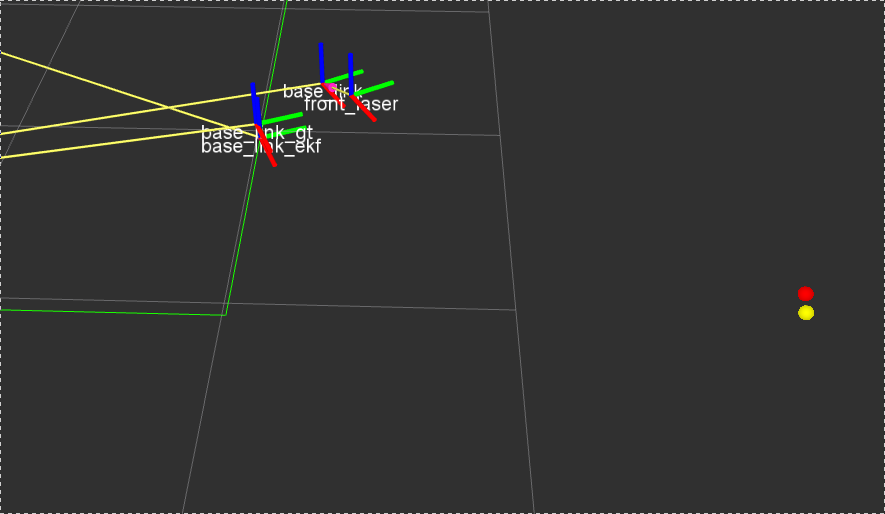
\includegraphics[width=\linewidth]{imagenesEKF/K1/4.png}
\endminipage
\end{figure}
\FloatBarrier

Trayectoria Efectiva:

\begin{figure}[!htb]
\begin{center}
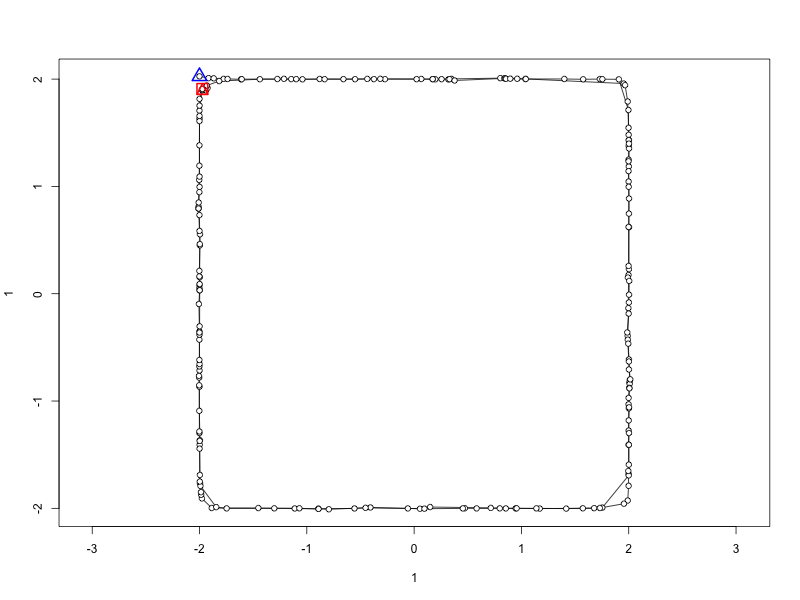
\includegraphics[width=\linewidth/2]{imagenesTrayectorias/ekf/ekf1.png}
\end{center}
\end{figure}
\FloatBarrier


Si bien el base\_link\_ekf continúa muy cercano al ground\_truth, podemos ver que base\_link ya para este caso diverge hacia un valor incorrecto.

Finalmente para $K=4$:

\begin{figure}[!htb]
\minipage{0.32\textwidth}
  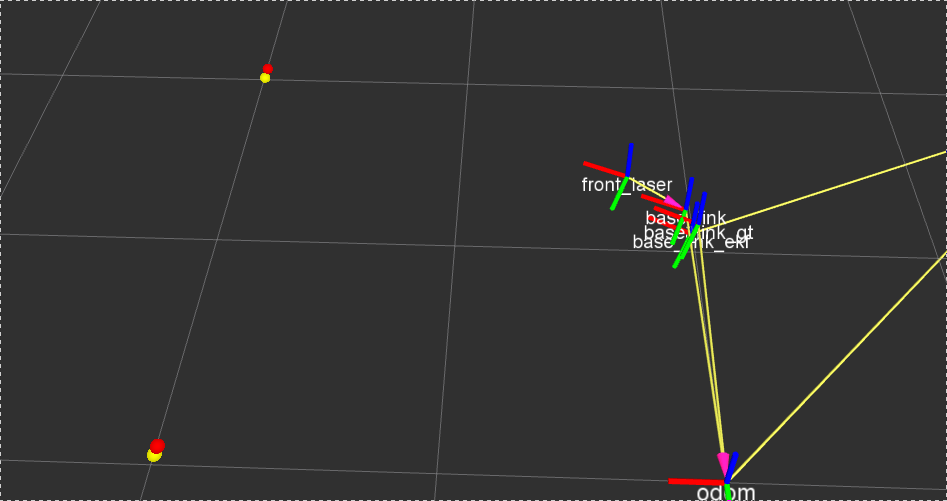
\includegraphics[width=\linewidth]{imagenesEKF/k4/1.png}
\endminipage\hfill
\minipage{0.32\textwidth}
  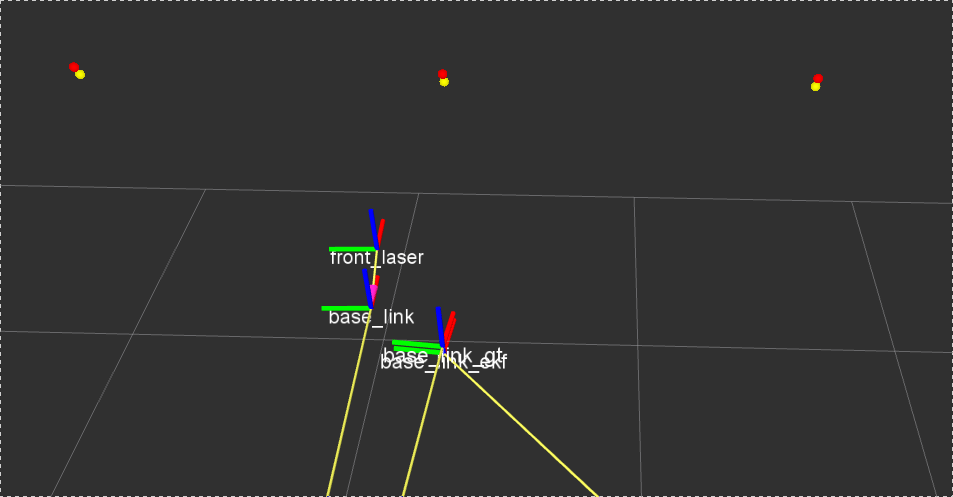
\includegraphics[width=\linewidth]{imagenesEKF/k4/2.png}
\endminipage\hfill
\minipage{0.32\textwidth}%
  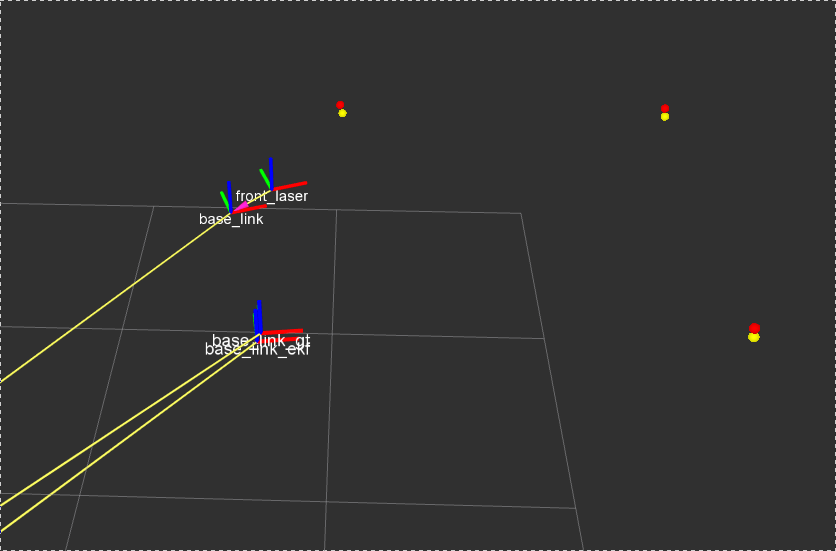
\includegraphics[width=\linewidth]{imagenesEKF/k4/3.png}
\endminipage
\end{figure}
\FloatBarrier

Trayectoria Efectiva:

\begin{figure}[!htb]
\begin{center}
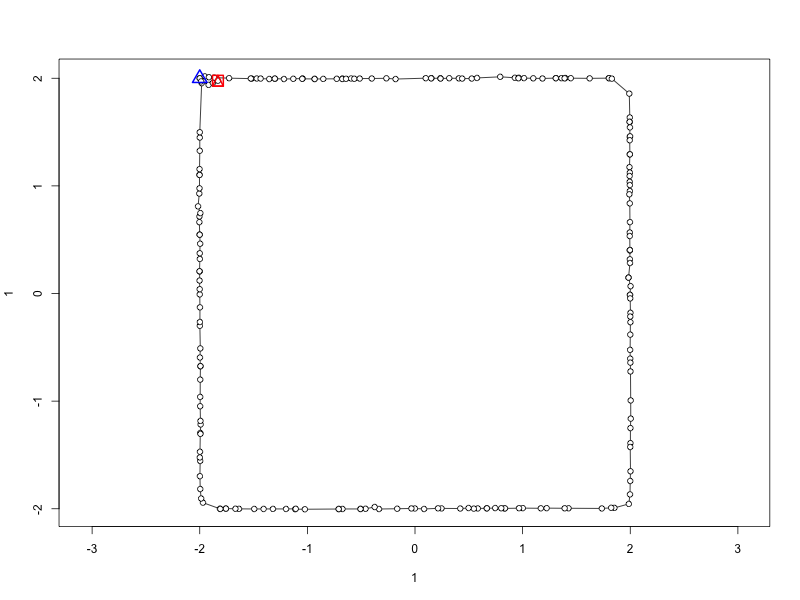
\includegraphics[width=\linewidth/2]{imagenesTrayectorias/ekf/ekf4.png}
\end{center}
\end{figure}
\FloatBarrier


%Comparativa de trayectorias entre lazo cerrado y lazo cerrado con EKF:

%concluciones: EKF te permite darle mucho mas velocidad sin perder precición, en cambio con lazo cerrado, si aumentas mucho la cte,

A diferencia del modelo previo de lazo cerrado Kalman permite estimar de manera muy precisa la pose real del robot aún para velocidades tan restrictivas.

En conclusión podemos apreciar que aplicando EKF es posible aplicar valores mucho mas restrictivos sobre la velocidad sin perder precisión en los valores odométricos. Si recordamos en el apartado de control a lazo cerrado esto no era posible ya que la acumulación de errores sistemáticos y del modelo cinemático en sí llevaba a estimaciones que no representaban de manera alguna la realidad.


%Utilizando como base los nodos provistos por la catedra hubo que hacer modificaciones sobre los siguientes paquetes:
%-lazo cerrado: adaptacion del modelo cinemático y control de feedback
%-robmovil_ekf: variante del modelo EKF del nuevo sistema
%-logger_node: nodo que fue necesario para conseguir los datos experimentales en  poses de los distintos marcos de referencia
%-alguno mas?

%-Para correr el sistema ejecutar las siguientes instrucciones:
%-catkin build
%-roscore
%-En este punto es recomendable levantar la escena de V-Rep 
%-source devel/setup.bash
%-catkin launch robmovil_ekf robmovil_ekf.launch 
%-Si va a usarse Rviz para algun tipo de analisis es necesario setear source sobre la carpeta contenedora el plugin.
\section{Conclusiones}
Como conclusiones finales de este trabajo se logró llevar a la práctica una gran cantidad de los conceptos vistos durante la cursada, a partir del análisis hecho sobre un nuevo modelo se pudo pasar de un sistema resuelto (modelo diferencial) a este que inicialmente resultaba una incógnita. 

A medida que implementamos los distintos componentes necesarios para conseguir el objetivo propuesto adquirimos conocimientos sumamente útiles sobre el sistema bajo estudio, la herramienta de desarrollo y temas anteriormente abordados (cinemática, seguimiento de trayectorias, filtro de kalman), consideramos que el aprendizaje de esto resulta muy enriquecedor 

Centrándonos en los resultados observamos que nuestra implementación presenta buenos resultados y en varias trayectorias no triviales se logró la navegación autónoma dentro del entorno simulado. La experimentación nos permitió ver los atributos que, en su correcta implementación, cada una de las partes partícipes en el sistema (Controlador de posición, seguidor de trayectoria, localizador de Kalman, etc) aportan tanto por separado y funcionando en conjunto.

%Hay algo mas para poner? Como por ejemplo cosas que no habia que hacer pero se pueden mejorar/agregar al TP? 

\section{Apendice}

\subsection{Detalles del sistema desarrollado}

Para concluir el trabajo presentamos un pantallazo general de todos los nodos trabajando en conjunto:

\begin{figure}[!htb]
\begin{center}
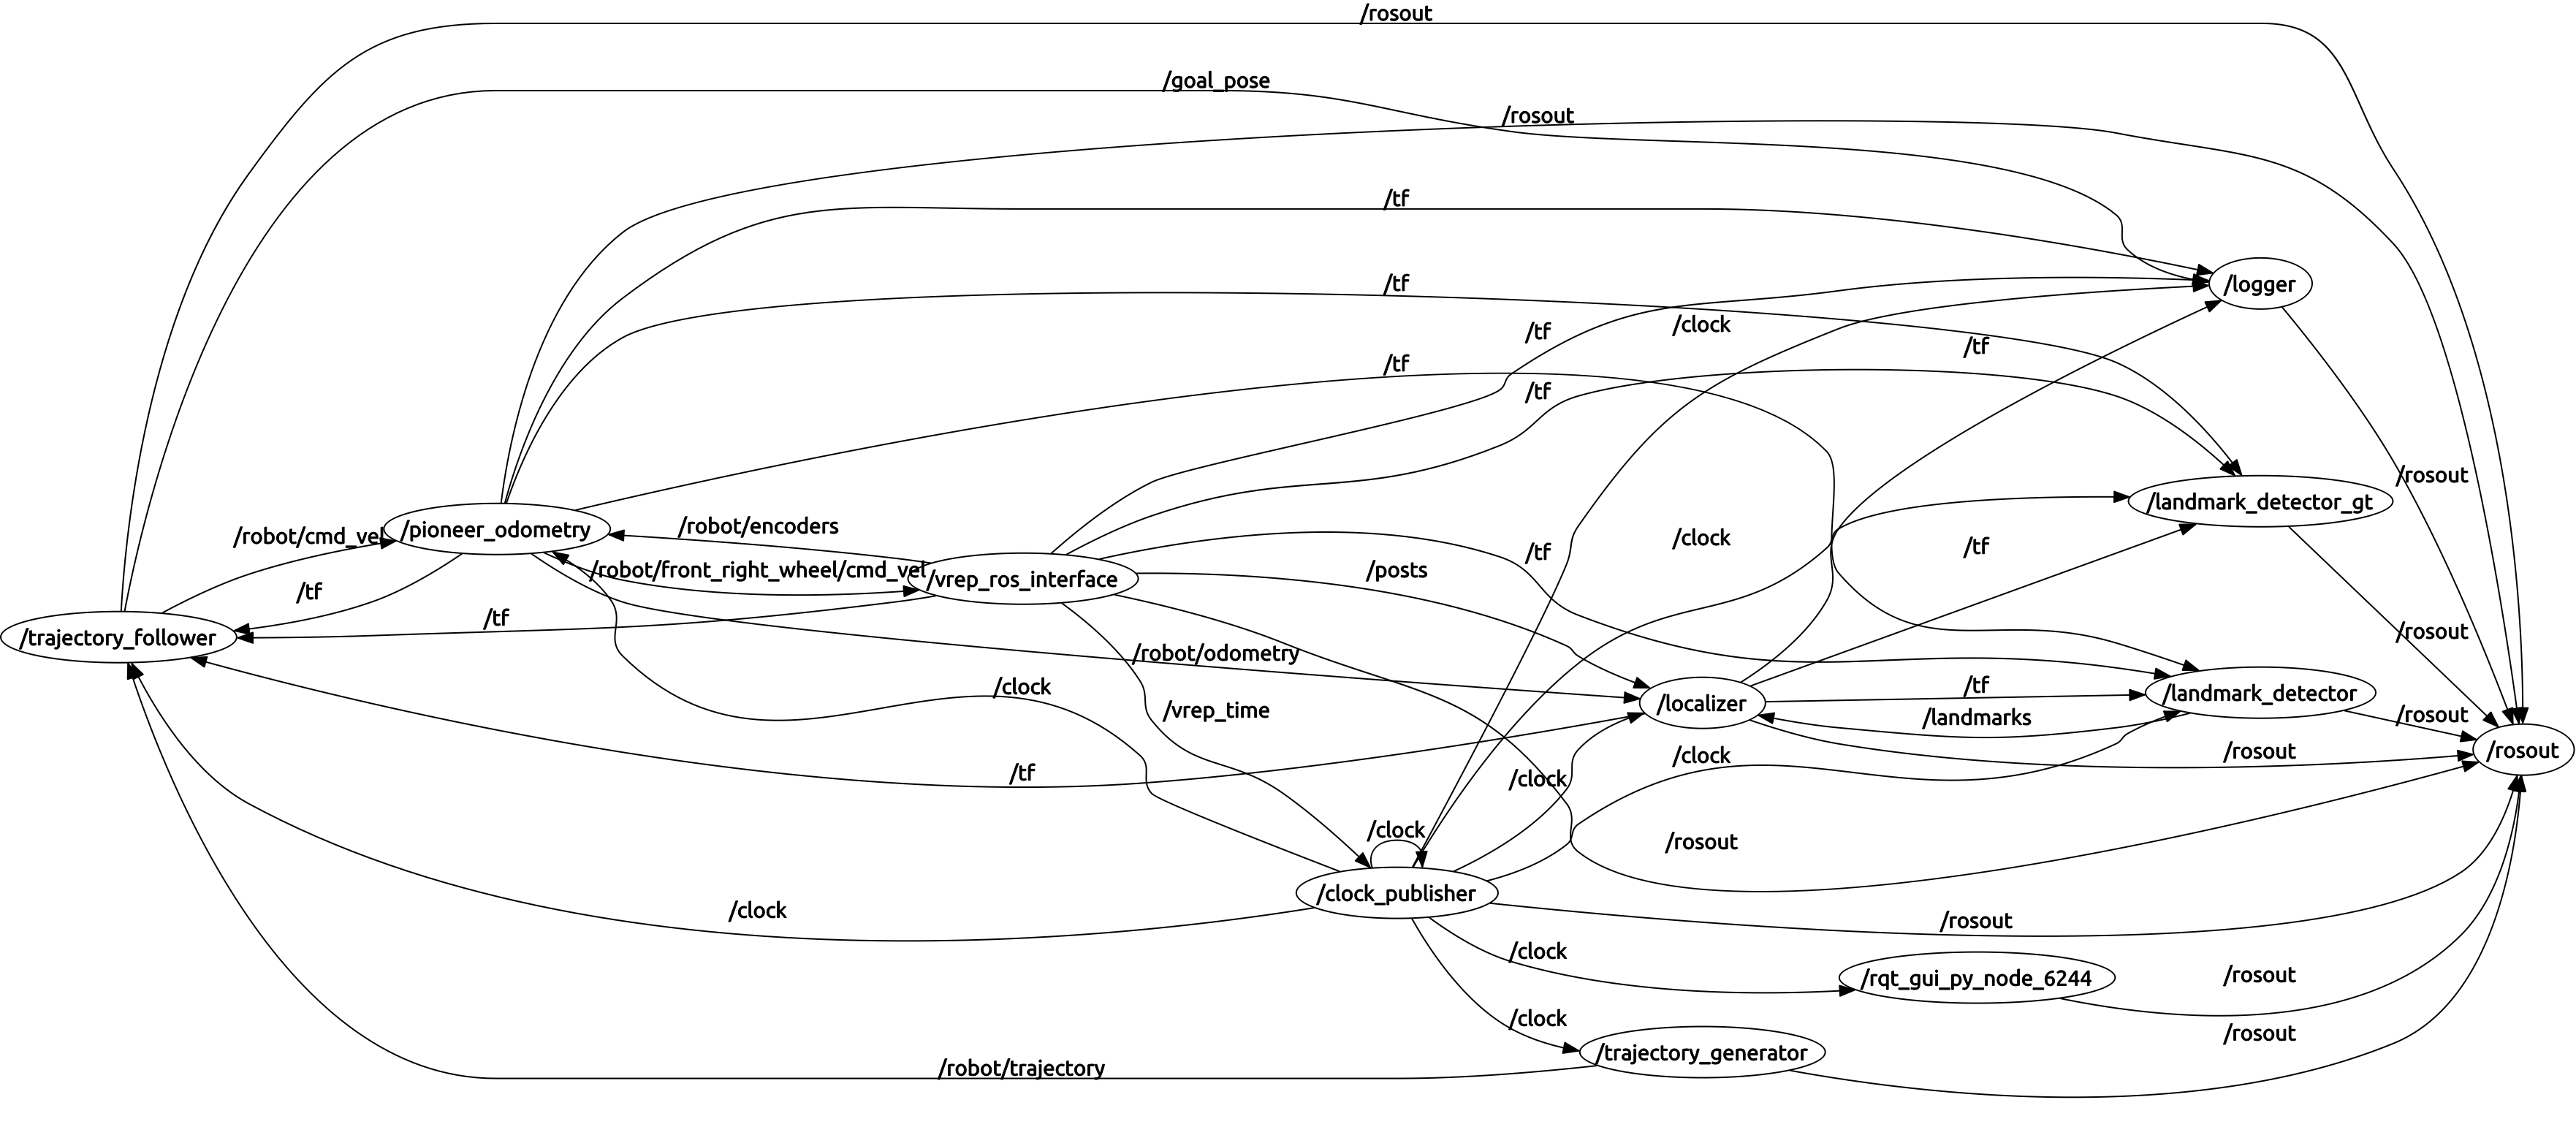
\includegraphics[width=\linewidth]{rqtgraphekf.png} 
\end{center}
\end{figure}

Sobre esta gran cantidad de mensajes siendo intercambiados en paralelo podemos destacar como lo más relevante al problema los siguientes:

El nodo encargado de la odometría recibe la información de los comandos de velocidad t encoders para enviar su estimación de la pose, esta es capturada por el "trajectory follower" que mide la distancia a la pose del goal juntando esto con lo recibido por el "trajectory generator" y publicando las consignas de velocidades necesarias para avanzar hacia el goal.

Por su parte el nodo "localizer" se suscribe a los tópicos de odometría, la información de senado y la ubicación del robot y postes en el simulado, con esto obtiene las consignas de covarianza y publica las transformaciones desde el marco EKF al del robot.

Por último el detector de landmarks de la IMU usa la información usa la información de scanning para actualizar la información de distancia respecto a los "landmarks".

\end{document}

